% !LW recipe=pdflatex only
\documentclass[aspectratio=169]{beamer}

% ---------- Packages ----------
\usepackage[utf8]{inputenc}
\usepackage[T1]{fontenc}
\usepackage{graphicx}
\usepackage{amsmath}
\usepackage{amssymb}
\usepackage{hyperref}
\usepackage{pifont}
\usepackage{booktabs}
\usepackage{xcolor}
\usepackage{colortbl}

\newcommand{\cmark}{\textcolor{green!50!black}{\ding{51}}}
\newcommand{\xmark}{\textcolor{red!70!black}{\ding{55}}}
\DeclareMathOperator*{\argmin}{arg\,min}
\newcommand{\Lloss}{\mathcal{L}}

% ---------- Theme ----------
\usetheme{Madrid}
\usecolortheme{default}

\definecolor{TPBordeaux}{RGB}{140,30,45}
\setbeamercolor{structure}{fg=TPBordeaux}
\setbeamertemplate{navigation symbols}{}

\AtBeginSection[]{
  \begin{frame}[plain,noframenumbering]
    \vfill
    \centering
    \usebeamerfont{title}\insertsectionhead\par
    \vfill
  \end{frame}
}

% ---------- Title info ----------
\title[Research Project RECH202]{Modèle de fondation pour l'EEG : pré-entraînement JEPA}
\author{Yanic ROTHLINGSHOFER}
\institute[]{\large \it Télécom Paris}
\date{\underline{Supervisor :} Van Tam Nguyen}

\begin{document}

\begin{frame}
  \titlepage
\end{frame}

\begin{frame}{Plan}
  \tableofcontents
\end{frame}

% ======================================================================
\section{Modèles de fondation pour l'EEG}
% ======================================================================

\begin{frame}{I-JEPA --- prédiction dans l'espace des représentations}
  \begin{columns}[T]
    \begin{column}{0.52\textwidth}
      \centering
      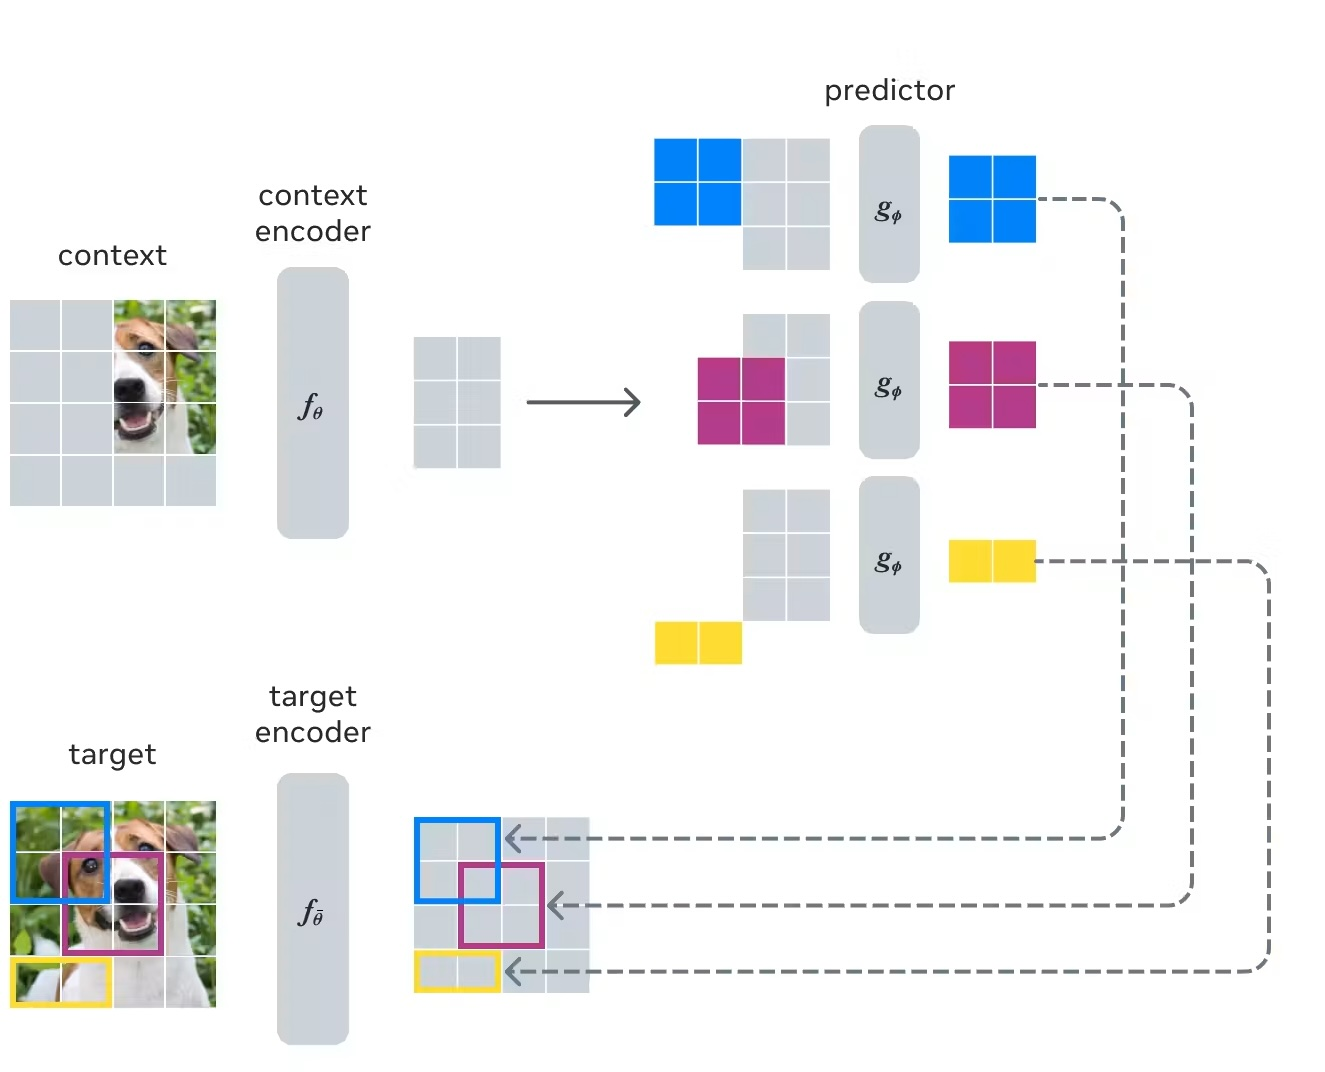
\includegraphics[width=\linewidth,height=0.62\textheight,keepaspectratio]{figures/i_jepa.jpg}
    \end{column}
    \begin{column}{0.46\textwidth}
      {\footnotesize
      Un \emph{context encoder} $f_\theta$ encode un bloc de contexte ; un \emph{target encoder}
      $f_{\bar\theta}$ (EMA de $f_\theta$) encode plusieurs blocs cibles. Un \emph{predictor}
      $g_\phi$, conditionné par les tokens de position des cibles, prédit leurs représentations :
      \[
        \Lloss_{\text{I-JEPA}}
        = \sum_{b} \big\| g_\phi\!\left(f_\theta(x_{\text{ctx}}),\, p_b\right) - \mathrm{sg}\big[f_{\bar\theta}(x_b)\big] \big\|_2^2
      \]
      \begin{itemize}
        \item \cmark\ Pas de reconstruction pixel/signal : cible sémantique, pas de détail haute fréquence.
        \item \cmark\ Pas de paires négatives, pas d'augmentations lourdes.
        \item \xmark\ Anti-collapse purement \emph{architectural} : EMA + \texttt{stop-grad} + asymétrie.
        \item \xmark\ Beaucoup d'hyperparamètres couplés (momentum, taille des blocs, \emph{warm-up}).
      \end{itemize}}
    \end{column}
  \end{columns}
\end{frame}


\begin{frame}{EEGPT --- masquage spatio-temporel et double objectif}
  \centering
  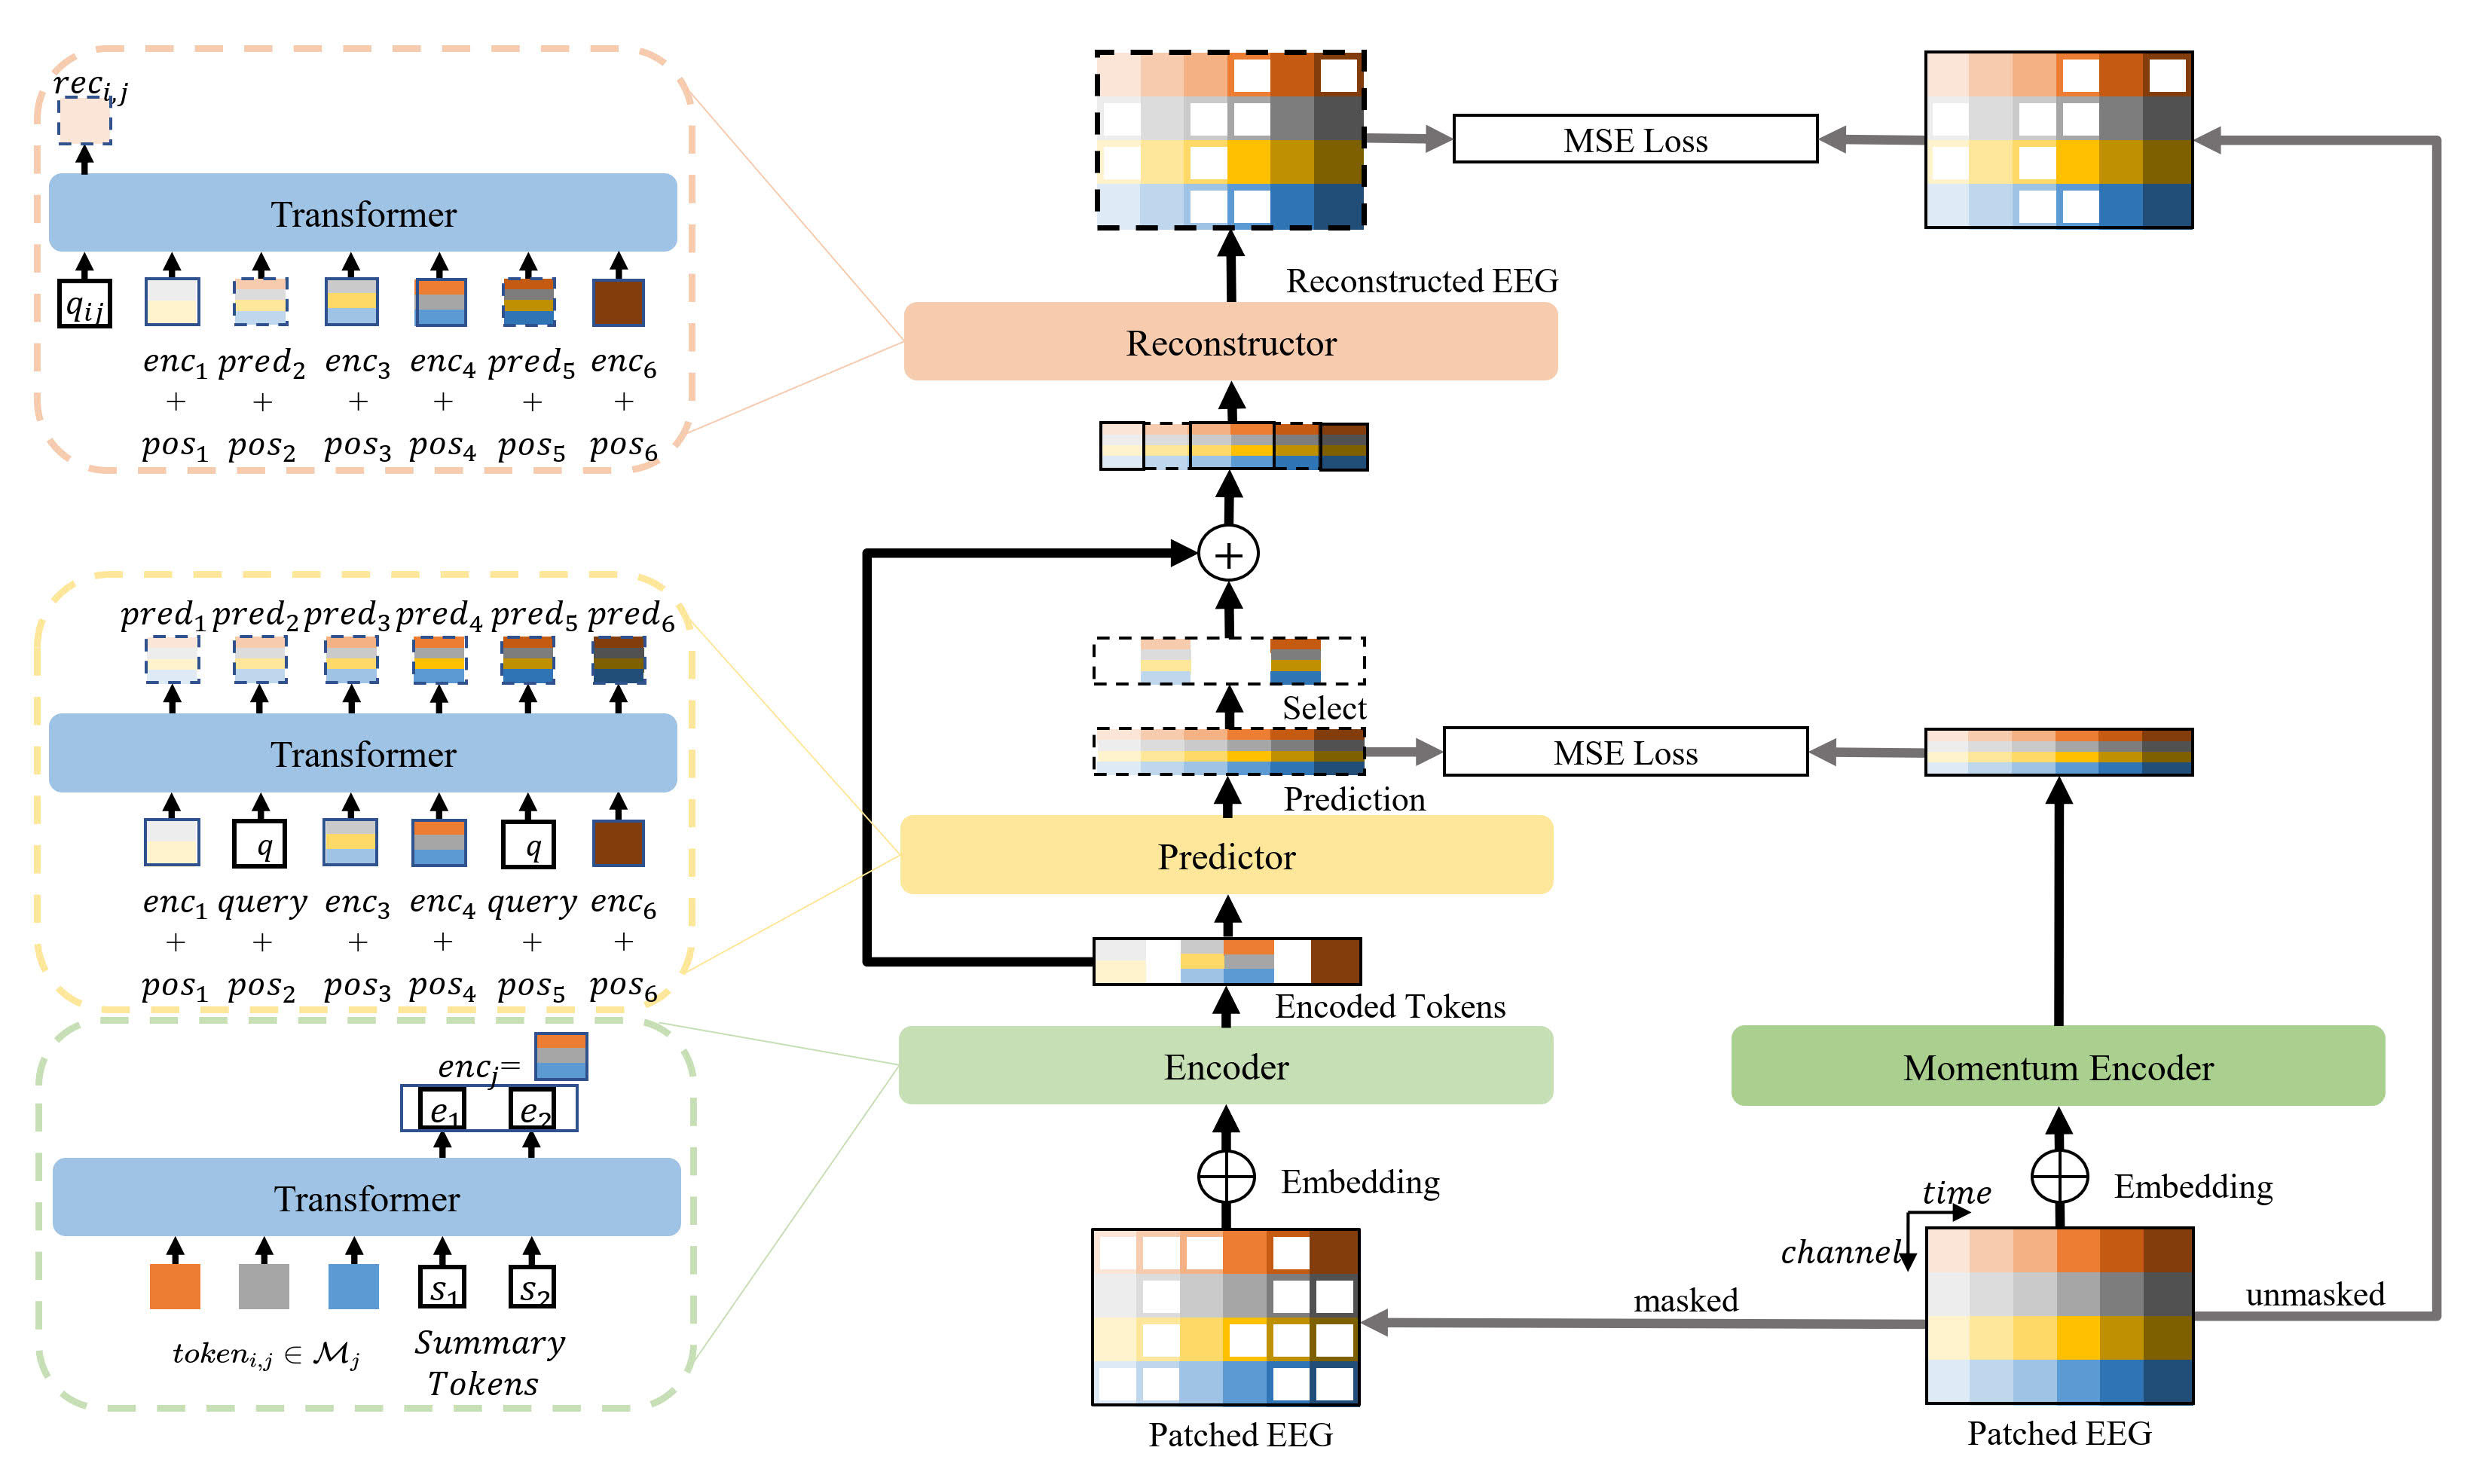
\includegraphics[width=\linewidth,height=0.85\textheight,keepaspectratio]{figures/EEGPT.jpg}
\end{frame}

\begin{frame}{REVE --- encodage spatio-temporel 4D et montages hétérogènes}
  \centering
  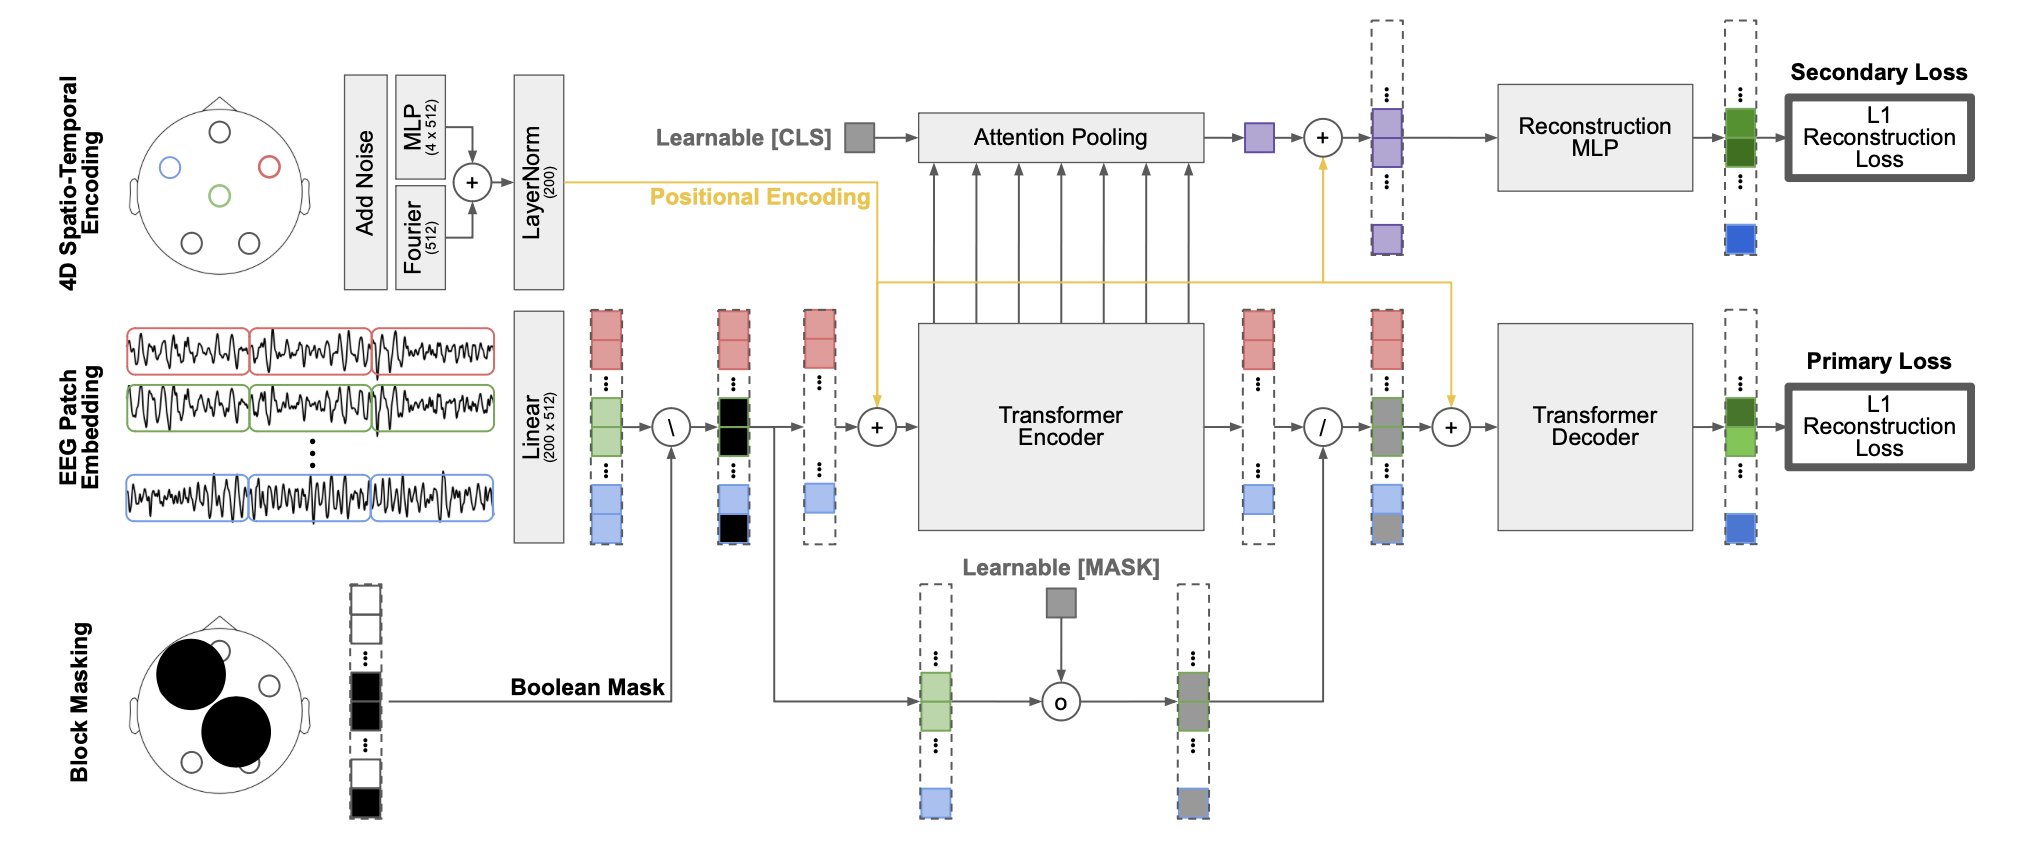
\includegraphics[width=\linewidth,height=0.85\textheight,keepaspectratio]{figures/reve.png}
\end{frame}

% ======================================================================
\section{Paradigme de pré-entraînement}
% ======================================================================

\begin{frame}
  \frametitle{LeJEPA --- 1. perte d'alignement}
  \textbf{Mise en place.} Un \textbf{seul} encodeur $f_\theta$, ni EMA, ni \emph{predictor}, ni \texttt{stop-grad}.
  Pour chaque signal $x_i$ du batch on tire $V$ vues globales et $L$ vues locales
  (bruit, échelle globale et par canal, décalage temporel, masques temps / fréquence / canaux) :
  \[
    z_i^{(u)} = f_\theta\big(x_i^{(u)}\big) \in \mathbb{R}^D,
    \qquad u = 1,\dots,V{+}L
  \]
  ($z_i^{(u)} = z_{\text{glob}}$, la sortie \emph{attention pooling} du bottleneck.)

  \vspace{0.15cm}
  \textbf{Objectif.} Toutes les vues d'un même signal doivent converger vers le centre de ses vues globales :
  \vspace{-0.1cm}
  \[
    c_i = \frac{1}{V}\sum_{v=1}^{V} z_i^{(v)},
    \qquad
    \Lloss_{\text{align}}
    = \frac{1}{B\,(V{+}L)\,D}\sum_{i=1}^{B}\ \sum_{u=1}^{V+L}
      \big\| z_i^{(u)} - c_i \big\|_2^2
  \]

  \vspace{0.1cm}
  {\footnotesize
  \begin{itemize}
    \item Le centre $c_i$ n'utilise que les vues \emph{globales} : les vues locales sont tirées vers elles,
          jamais l'inverse.
    \item $c_i$ n'est pas détaché $\Rightarrow$ le gradient circule dans toutes les vues (aucune asymétrie).
    \item Seule, cette perte est minimisée par la solution triviale $z \equiv \text{const}$ : d'où la
          régularisation.
  \end{itemize}}
\end{frame}

\begin{frame}
  \frametitle{LeJEPA --- 2. perte de régularisation (SIGReg)}
  \textbf{Objectif.} Forcer la distribution des $z$ \emph{dans le batch} à être une gaussienne isotrope
  $\mathcal{N}(0, I_D)$. Test fait sur des projections 1D (\emph{sketching}) :
  $S$ directions $\theta_s \sim \mathcal{U}(\mathbb{S}^{D-1})$, puis comparaison de la fonction
  caractéristique empirique de $\langle \theta_s, z\rangle$ à celle de la gaussienne, $e^{-t^2/2}$ :
  \vspace{-0.1cm}
  \[
    \hat\varphi_s(t) = \frac{1}{B}\sum_{i=1}^{B} e^{\mathrm{i}\,t\,\langle \theta_s,\, z_i\rangle},
    \qquad
    \Lloss_{\text{SIGReg}}
    = \frac{1}{S}\sum_{s=1}^{S} B \int_{-5}^{5}
      \big|\hat\varphi_s(t) - e^{-t^2/2}\big|^2\, \underbrace{e^{-t^2/2}}_{\text{poids}}\,\mathrm{d}t
  \]

  \vspace{0.1cm}
  \textbf{Objectif total}, un unique hyperparamètre $\lambda$ :
  \vspace{-0.1cm}
  \[
    \Lloss = (1-\lambda)\,\Lloss_{\text{align}} + \lambda\,\Lloss_{\text{SIGReg}},
    \qquad \lambda = 0.05
  \]

  \vspace{-0.1cm}
  {\footnotesize
  \begin{itemize}
    \item En pratique : $S = 256$ directions, intégrale par trapèzes sur $17$ points de $[-5,5]$,
          calculée en \texttt{float32} et sommée sur les GPU en DDP.
    \item Directions retirées à chaque pas depuis \texttt{base\_seed}$+$\texttt{global\_step} :
          identiques sur tous les rangs, mais renouvelées à chaque itération.
    \item Appliquée séparément à chaque vue, puis moyennée sur les $V{+}L$ vues.
  \end{itemize}}
\end{frame}

\begin{frame}{LeJEPA --- pourquoi ce choix}
  \begin{columns}[T]
    \begin{column}{0.5\textwidth}
      \textbf{Avantages}
      \begin{itemize}
        \item \cmark\ Anti-collapse \emph{explicite} : SIGReg interdit toute distribution dégénérée,
              plus besoin d'EMA, de \texttt{stop-grad} ni de \emph{predictor}.
        \item \cmark\ Un seul hyperparamètre de perte ($\lambda$).
        \item \cmark\ La gaussienne isotrope est le prior qui minimise le risque du \emph{probing}
              linéaire en aval.
        \item \cmark\ Coût $\mathcal{O}(B\,S\,P)$ par vue : négligeable devant l'encodeur.
      \end{itemize}
    \end{column}
    \begin{column}{0.5\textwidth}
      \textbf{Limites / points de vigilance}
      \begin{itemize}
        \item \xmark\ SIGReg est une statistique \emph{sur le batch} : elle exige un batch large
              (à $B=4$ le latent collapse).
        \item \xmark\ Les vues doivent rester informatives : des gains d'augmentation nuls
              annulent la diversité des vues globales.
        \item \xmark\ Invariance imposée par les augmentations : si elles effacent
              l'information de tâche, elle disparaît du latent.
      \end{itemize}
    \end{column}
  \end{columns}

  \vspace{0.2cm}
  {\footnotesize Valeurs de référence en régime sain : $\Lloss_{\text{SIGReg}} \approx 1.06$,
  $\Lloss_{\text{align}} \approx 1.17$.}
\end{frame}

% ======================================================================
\section{Résultats et analyse}
% ======================================================================

\begin{frame}
  \frametitle{Analyse du latent global par PCA --- BCI2A (imagerie motrice, 4 classes)}
  \centering
  \vfill
  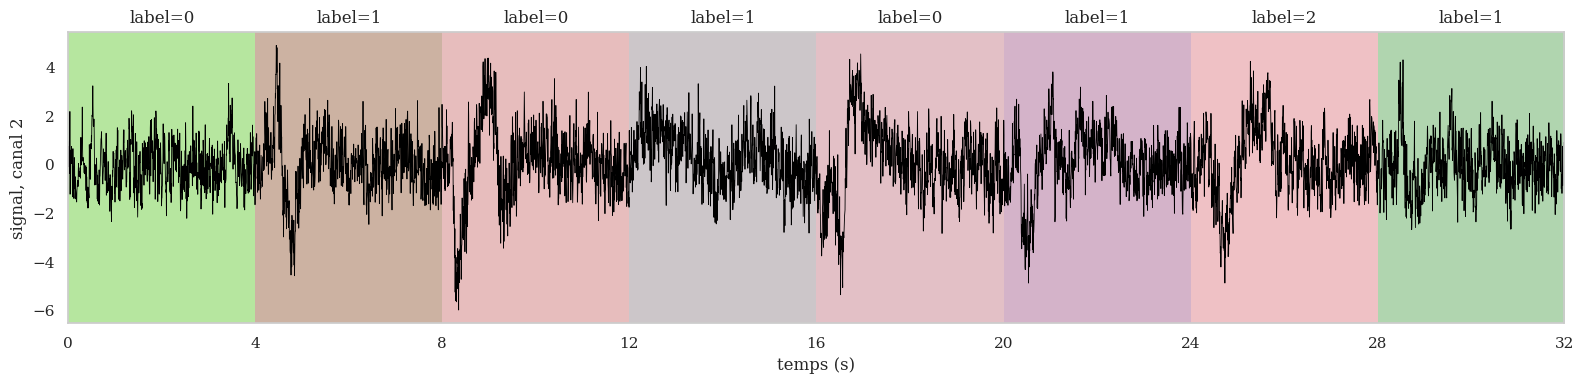
\includegraphics[width=\linewidth]{figures/output.png}

  \vfill
  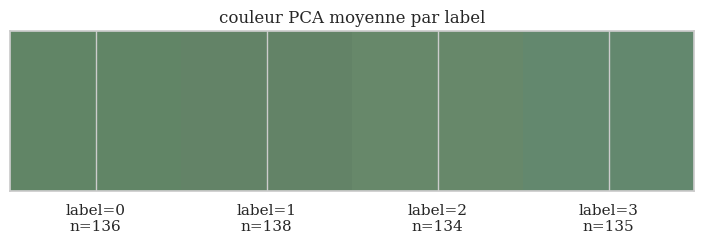
\includegraphics[width=0.52\linewidth]{figures/pca_glob.png}
  \vfill
\end{frame}

\begin{frame}{Comparaison aux modèles de l'état de l'art --- balanced accuracy (\%)}
  \centering
  \vfill
  \renewcommand{\arraystretch}{1.25}
  \resizebox{\linewidth}{!}{%
  \begin{tabular}{l c ccccc}
    \toprule
    \textbf{Modèle} & \textbf{\#params (M)}
      & \textbf{BCI2A} & \textbf{PHYSIONETMI} & \textbf{FACED} & \textbf{SLEEPEDF} & \textbf{TUAB} \\
    \midrule
    CBraMod   & -- & -- & -- & -- & -- & -- \\
    CSBrain   & -- & -- & -- & -- & -- & -- \\
    EEGMamba  & -- & -- & -- & -- & -- & -- \\
    EEGPT     & -- & -- & -- & -- & -- & -- \\
    LaBraM    & -- & -- & -- & -- & -- & -- \\
    REVE      & -- & 63.62 & \textbf{63.01} & \textbf{54.42} & -- & -- \\
    LuMamba   & -- & -- & -- & -- & -- & -- \\
    LUNA      & -- & -- & -- & -- & -- & -- \\
    \midrule
    \rowcolor{TPBordeaux!12}
    \textbf{EEG-FM (ours)} & -- & -- & -- & -- & -- & -- \\
    \midrule
    EEGNet \emph{(baseline)} & -- & \textbf{72.66} & 60.46 & 49.67 & -- & -- \\
    \bottomrule
  \end{tabular}}
  \vfill
\end{frame}

\end{document}
